\documentclass[sigconf,authorversion,nonacm]{acmart}
\usepackage{graphicx} % Required for inserting images
\usepackage{amsmath,amsfonts,amsthm} % Math packages
\usepackage{float}

%\usepackage[hmarginratio=1:1,top=32mm,left=18mm,columnsep=20pt]{geometry} % Document margins

\usepackage[style=ieee, backend=bibtex]{biblatex}
\addbibresource{references.bib}

\title{CSC586C-Report 1}
\author{Steven Bobyn \and Tyler Makaro \and Zhixin Fang}
\date{\today}

\settopmatter{printfolios=true}

\begin{document}

\begin{abstract}
  To understand how to apply GPU programming techniques to Deep Learning, we train a simple Deep Neural Network using CUDA to classify images of digits from the MNIST dataset. In this milestone, we provide a full implementation of the network and training process in Python using NumPy with SIMD optimization, a C++ implementation of forward propagation with no parallel programming, and a CUDA implementation of forward propagation that successfully exposes some simple data-level parallelism. Currently, our CUDA implementation is slower than our reference C++ implementation. However, we have identified weaknesses in our use of GPU memory and opportunities for further data-level parallelism that can be addressed in the following milestones to improve our results.
  
  \end{abstract}

\maketitle

\section{Introduction}
Deep Learning (DL) has seen dramatic success over the past decade. Much of this success is often attributed to the availability of GPU hardware and software suited to computing inherently parallel tasks in training Deep Neural Networks (DNNs) with large amounts of data. Our group consists of three Master's students with mathematical backgrounds interested in DL; with this project, we want to better understand how the GPU can be leveraged in DL problems. We have limited the scope of our project to training a three-layer multi-layer perceptron \cite{perceptron} on the classic MNIST dataset \cite{mnist}.

This limited scope in the field of Deep Learning allows us to focus our attention on the aspects of Deep Learning that most pertain to GPU Programming. Moreover, the MLP network is ubiquitous in DNN architectures from Convolutional Networks \cite{alexnet} to Transformers \cite{transformer}, so our findings and intuitions developed in this project will generalize widely. Our choice of problem, classification on the MNIST dataset, is a classic example in the field, and it is small enough to train within minutes on a modern CPU; this makes it well-suited for iterating and testing our work, while still having plenty of opportunity for data-level parallelism having 60,000 training example, each being a 784-dimensional vector of floats.

\section{Theory}

We will start by defining the structure of our network. We use a structure similar to that described by 3Blue1Brown's excellent video\cite{3b1b}. The network will consist of 4 layers, an input layer of 784 neurons that takes a flattened image with each grey scale pixel scaled from 0 to 1; two internal layers of $k_1$ and $k_2$ neurons; and an output layer of 10 neurons. We can define the forward propagation between layers as:

\begin{figure}
    \centering
    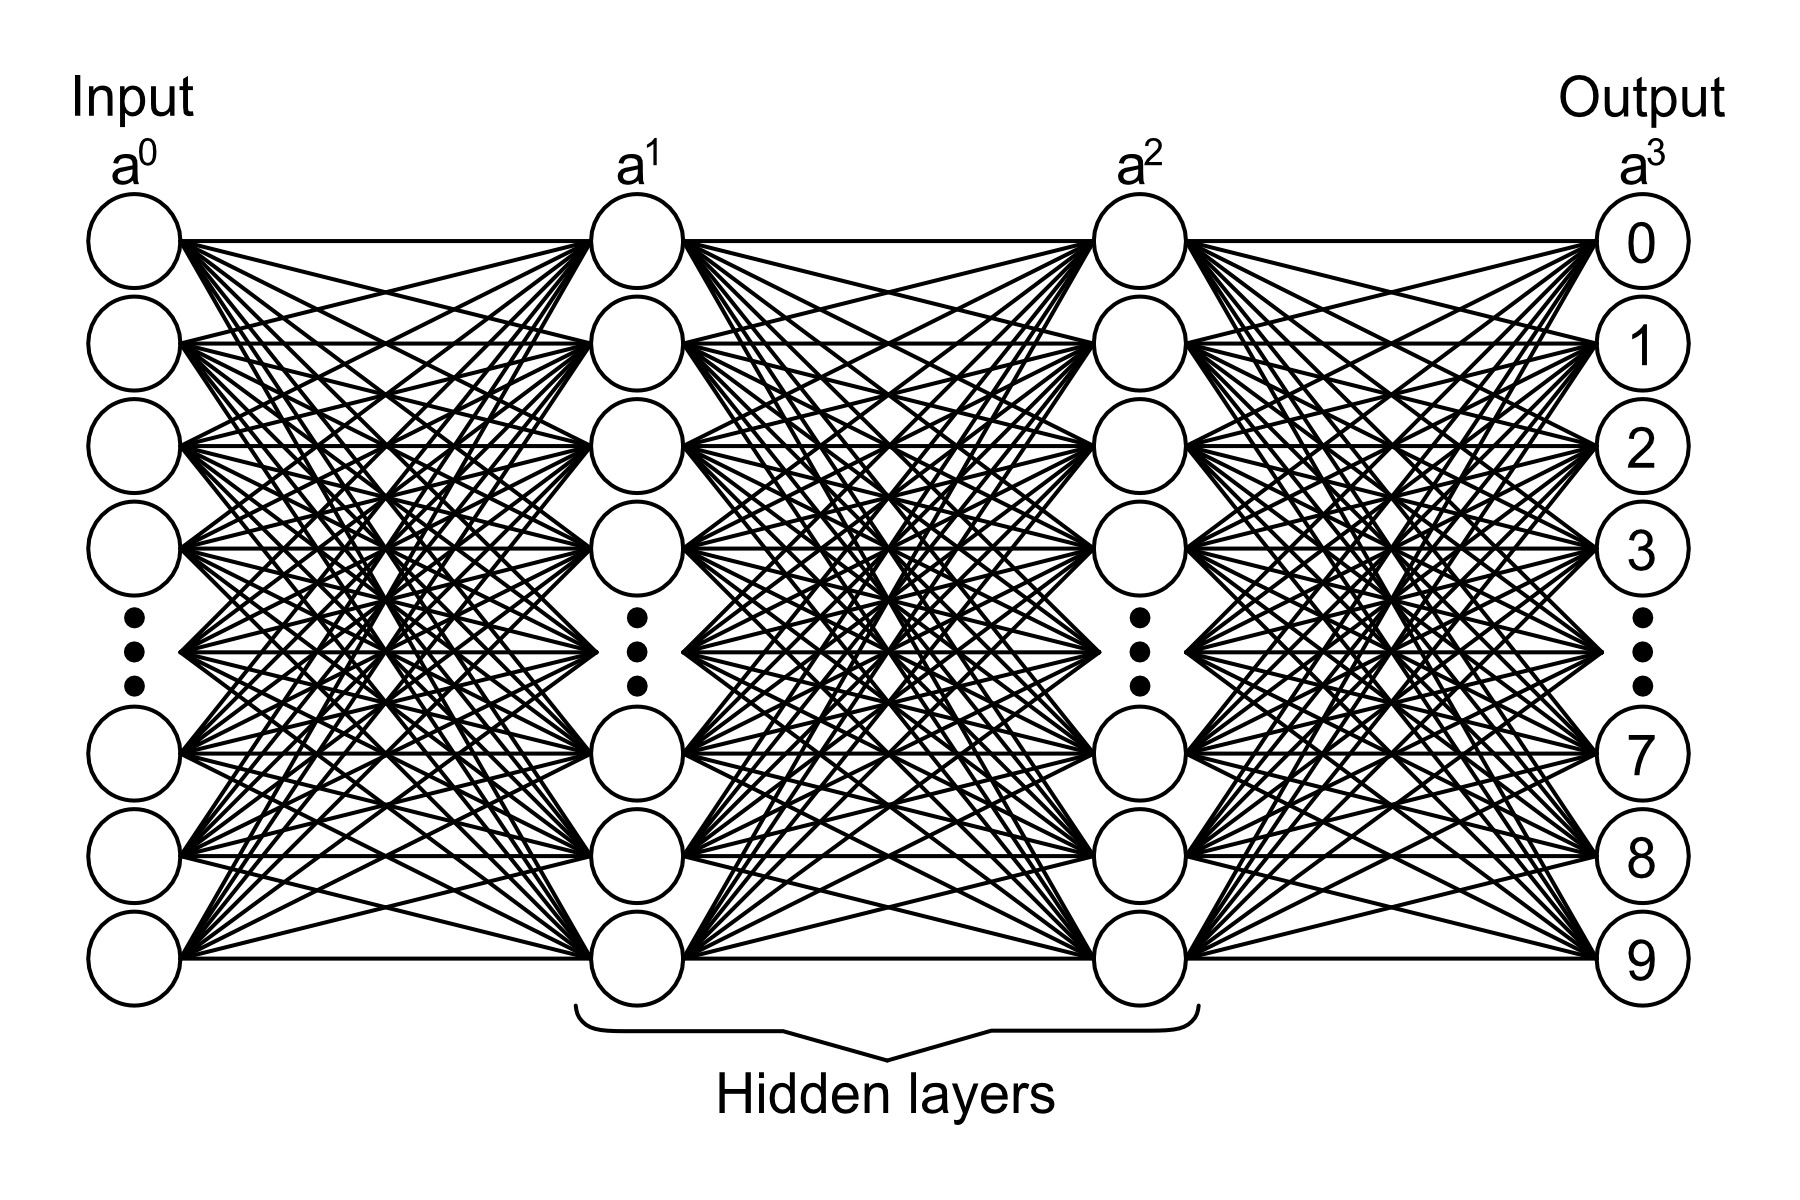
\includegraphics[width=0.9\linewidth]{images/nn.png}
    \caption{multi-layer perceptron}
    \label{fig:nn}
\end{figure}

\begin{equation}
    \vec{z}^L = w^{L-1}\vec{a}^{L-1}+\vec{b}^{L-1}
    \label{eq:forward-propagation-z}
\end{equation}

\begin{equation}
    \vec{a}^L = \sigma(\vec{z}^L)
    \label{eq:forward-propagation}
\end{equation}

Where $\vec{a}^0$ is the input image and where $\vec{a}^L$ is the vector of activations of the neurons in the $L^{th}$ layer, $w^L$ and $\vec{b}^L$ are the corresponding weights and biases of appropriate shape, and $\sigma$ is the sigmoid \eqref{eq:sigmoid} function applied element-wise. The predicted output of the network is the index of $\vec{a}^3$ with the highest output. The weights and biases will be initialized with noise from a normal distribution.

\begin{equation}
    \sigma(x) = \frac{1}{1+e^{-x}}
    \label{eq:sigmoid}
\end{equation}

Dropping the $\vec{ }$\hspace{2pt} from here on, we have as  well:
\begin{align*}
    a^0&\in\mathbb{R}^{784} \\
    w^0&\in\mathbb{R}^{784\times k_1} \\
    b^0, a^1&\in\mathbb{R}^{k_1}\\
    w^1&\in\mathbb{R}^{k_1\times k_2} \\
    b^1, a^2&\in\mathbb{R}^{k_2}\\
    w^2&\in\mathbb{R}^{k_2\times 10} \\
    b^2, a^3&\in\mathbb{R}^{10}\\
\end{align*}


\subsection{Training}

We train the model with mini-batch gradient descent and back-propagation. The MNIST dataset contains 70,000 images each of 28x28 pixels (flattened to 784 pixels) with a corresponding label indicating the target digit. We use the first 60,000 images for training, and the remaining 10,000 images for testing the model. With enough training time this model should be able to reach $\geq 93\%$ accuracy rather easily.

Computing the gradient will be done in batches of size $n$ from a random (fixed seed) sample of images, and averaging these together before updating weights and biases. This provides opportunity for parallelism of not only the matrix-vector multiplication on the GPU but also the computation of each per-sample gradient.

We will use a cross entropy cost function \cite{entropy-cost-f} which we can define for a single training instance as:
\begin{equation}
    C = -\sum_{i=0}^9(y_i\ln{a^3_i}+(1-y_i)\ln(1-a^3_i))
\end{equation}
where $y_i$ is a component of the one-hot vector encoding a 1 at index i for an image of digit i. We are only ever interested in the gradient of the cost function, so we have:
\begin{equation}
    \frac{\partial C}{\partial a^3_i} = \frac{a_i^3-y_i}{a_i^3(1-a_i^3)}
\end{equation}
from here we can back-propagate. To help us find the gradient of the cost with respect to the weights and biases we first find the derivative of the cost with respect to neurons in the previous layer by:
\begin{equation}
    \frac{\partial C}{\partial a^{L-1}_k} = \sum_{j=0}^{k-1} w^{L-1}_{jk} \sigma'(z^L_j) \frac{\partial C}{\partial a^{L}_j}
\end{equation}
We then compute the gradient with respect to the weights and biases as:
\begin{equation}
    \frac{\partial C}{\partial b^{L-1}_{j}} = \sigma'(z^L_j) \frac{\partial C}{\partial a^{L}_j}
\end{equation}
and
\begin{equation}
    \frac{\partial C}{\partial w^{L-1}_{jk}} = a^{L-1}_k \sigma'(z^L_j) \frac{\partial C}{\partial a^{L}_j}
\end{equation}
This gives us $\nabla_wC$ and $\nabla_bC$.

Abusing notation a bit, we compute these for a few samples and update the weights and biases by:
\begin{equation}
    w,b = w,b - \alpha \frac{1}{n}\sum_{samples}\nabla_{w,b}C
\end{equation}
where $\alpha$ is the learning rate, and $n$ is the batch size. We repeat over the entire training set, and then we repeat that again for any number of epochs desired.

\section{Implementations}
Source code is available on GitHub\cite{CSC586C_Project}. Our environment is Windows 11 using Microsoft Visual Studio 2022 and CUDA toolkit 12.6 unless stated otherwise in a read me file in the repository.

\subsection{Python}
We have written a complete working implementation in Python using just NumPy and a few other supporting libraries for visualization and loading data. It's worth noting that since NumPy v1.20 that the library has widely expanded the use of SIMD instructions\cite{NumPyNotes}. This makes it entirely reasonable for our python implementation to perform as good if not better than our C++ implementation without SIMD.

This implementation contains code for both forward and backwards propagation. It also contains code to export randomised, and trained weights and biases to a csv file for import into our CUDA and C++ implementations for testing. Finally, we use an iPython notebook for interaction with the implementation.

\subsection{C++}
In order to assist the process of porting the Python implementation to CUDA, we have first ported the implementation over to C++ first. This is a single-threaded, no SIMD, implementation.

\subsection{CUDA}

We have two working CUDA implementation for forward propagation which we call "Stupid" and "Naive" respectively. 
\begin{itemize}
    \item "Stupid" solution exposes data level parallelism by doing matrix-vector multiplication and element-wise vector/matrix operations as 1 thread per output element. It uses small global kernels of operations, transferring data between host and device for each add/sigmoid/matmul operation creating a stupid amount of host-device transfers. We start from the reference C++ solution first, then essentially re-implemented each individual step in Formula (1) \& (2) in CUDA, and calls them from the host in a for-loop. This allows us to verify correctness.
    \item "Naive" implementation eliminates a large portion of host-device transfers. Since one forward layer is a chained call of a Matmul(), Add() and Sigmoid(), we can easily implement it by calling the three operations previously implemented in global kernels in device kernels.
\end{itemize}


The mindset behind completing a non-parallelized solution first is that we want to ensure the correctness for each step in a chained operation. Once we verified the correctness of each step, combining them to form a big kernel is trivial as long as we pass the data correctly. 

\subsection{Running the solution}

First, pull the release tagged "Report 1" from our git repo\cite{CSC586C_Project}. Then extract the data.zip directly. You should see a bunch of csv files directly in ./data/ folder.

The CUDA can be built using VS2022+CUDA12.6. Make sure to choose "Release" mode to get optimized host performance.

Note: The aforementioned "stupid" solution will not be used as our baseline. It's mainly there to provide step-by-step verification for our device kernels.

\section{Experiments}
We are using values of $k_1=k_2=300$, and a batch size of $n=10$. For the purposes of the following numbers, the single core implementations were run on an AMD Ryzen 5800X3D, and CUDA implementations were run on a single laptop NVidia RTX 4050.

\subsection{Forward Propagation}
Forward propagation is working, and achieves identical accuracy to the Python implementation when using the trained weights and biases from the Python implementation for both the C++ and CUDA implementations. The numbers were collected with the build set to release and not debug for better performance.

\begin{table}[H]
    \centering
    \begin{tabular}{ccc}
        Implementation & 10k time (s) & 60k time (s) \\ \hline
        Python & 0.5 & 2.9 \\
        C++ & 2.2 & 13.3 \\
        "Naive" CUDA & 11.5 & 67.44 \\
    \end{tabular}
    \caption{Runtime for forward pass on training and test data sets}
    \label{tab:my_label}
\end{table}

\begin{figure}[H]
    \centering
    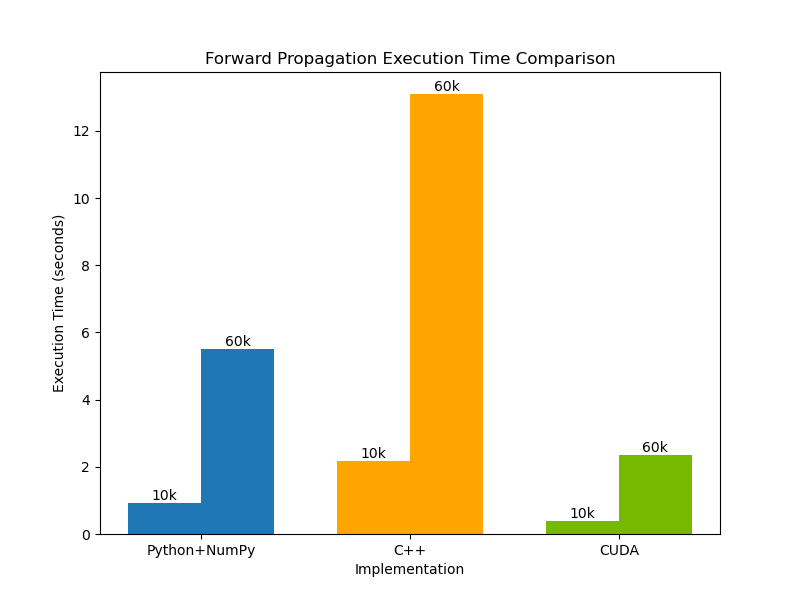
\includegraphics[width=0.9\linewidth]{images/forward_prop_time_comparison.png}
    \caption{Runtime for forward pass on training and test data sets}
    \label{fig:enter-label}
\end{figure}

\subsection{Backwards Propagation}
This is not yet finished on the C++ and CUDA implementations. But a single run of 6000 batches of 10 images each takes the python implementation approximately 1min 17s to run.

\section{Methods and Future Work}

We are continuing to implement CPU backward propagation in C++, and CUDA. Implementing back propagation will be completed in the next milestone.

Our approach of porting first to C++ then to CUDA allows us to start from smaller, easily verifiable kernels first, then start to expose data-level parallelism gradually by combining kernels that can be called on the device. This will allow us to minimize transfers between host and device until we ultimately have only transfers at the beginning and end of the computation. 

This could even upgraded with CUDA streams to begin processing the first batch of data in the back propagation before data transfer as completed. This could also be applied to running the forward propagation should we need to run the model before training (or if we wish to compare against the weights and biases exported from the python model).

\subsection{Data Level Parallelism}

Our use of data level parallelism could use a lot of improvements. We have some parallelism already in assigning different threads to work on different output elements of matrix/vector operations. Here is a list of the ones we are currently thinking of:
\begin{itemize}
    \item For forward propagation, we can do as many images in parallel with minimal syncing since each forward propagation is independent of another. This is limited largely by the available CUDA cores if done well.
    \item For backwards propagation, we can parallelise the computation of the gradient for each sample within a mini batch before averaging them together. This is largely limited by the batch size, so experimenting with larger batch sizes and appropriately larger learning rates will be useful.
    \item We should utilize shared memory. The weights matrix can be shared by the entire neural network, as opposed to being passed to the kernels for each layer. This will be most effective with parallelism described in the point above, as without mini-batch parallelism, much of the computation is unique from node to node and layer to layer.
\end{itemize}

The largest matrix that we are working with is 784x300 which, so we may see benefit from more than just a number of threads equal to the output object size. Passing part of a dot product to different cores and reducing is also worth trying.

Finally if time allows, using tensor cores for some of these matrix/vector operations may be beneficial if not at least interesting.

\subsection{Profiling}

In the first report, we simply use the chrono library to measure the execution time. We will include NSight profiling results in the future when we do backpropagation, as training will have significantly higher utilization.

\section{Conclusion}
Minimizing transfers between host and device and mini-batch-level parallelism are expected to significantly improve performance in the next milestone.

\printbibliography
\end{document}
